%% (Master) Thesis template
% Template version used: v1.4
%
% Largely adapted from Adrian Nievergelt's template for the ADPS
% (lecture notes) project.

\PassOptionsToPackage{dvipsnames}{xcolor}

%% We use the memoir class because it offers many easy to use features.
\documentclass[11pt,a4paper,titlepage]{memoir}

%% Packages
%% ========

%% LaTeX Font encoding -- DO NOT CHANGE
\usepackage[OT1]{fontenc}

%% Babel provides support for languages.  'english' uses British
%% English hyphenation and text snippets like "Figure" and
%% "Theorem". Use the option 'ngerman' if your document is in German.
%% Use 'american' for American English.  Note that if you change this,
%% the next LaTeX run may show spurious errors.  Simply run it again.
%% If they persist, remove the .aux file and try again.
\usepackage[american]{babel}

%% Input encoding 'utf8'. In some cases you might need 'utf8x' for
%% extra symbols. Not all editors, especially on Windows, are UTF-8
%% capable, so you may want to use 'latin1' instead.
\usepackage[utf8]{inputenc}

%% This changes default fonts for both text and math mode to use Herman Zapfs
%% excellent Palatino font.  Do not change this.
\usepackage[sc]{mathpazo}

%% The AMS-LaTeX extensions for mathematical typesetting.  Do not
%% remove.
\usepackage{amsmath,amssymb,amsfonts,mathrsfs}

%% NTheorem is a reimplementation of the AMS Theorem package. This
%% will allow us to typeset theorems like examples, proofs and
%% similar.  Do not remove.
%% NOTE: Must be loaded AFTER amsmath, or the \qed placement will
%% break
\usepackage[amsmath,thmmarks]{ntheorem}

%% LaTeX' own graphics handling
\usepackage{graphicx}
\graphicspath{{figures/}} %tell package where to find graphics


%% We unfortunately need this for the Rules chapter.  Remove it
%% afterwards; or at least NEVER use its underlining features.
\usepackage{soul}

%% This allows you to add .pdf files. It is used to add the
%% declaration of originality.
\usepackage{pdfpages}

\usepackage{xspace}

\usepackage{capt-of}

\usepackage{float}

\usepackage[section]{placeins}

\usepackage{subfig}

\usepackage[square, comma, sort&compress, numbers]{natbib}
%% Some more packages that you may want to use.  Have a look at the
%% file, and consult the package docs for each.
%% See the TeXed file for more explanations

%% [OPT] Multi-rowed cells in tabulars
%\usepackage{multirow}

%% [REC] Intelligent cross reference package. This allows for nice
%% combined references that include the reference and a hint to where
%% to look for it.
\usepackage{varioref}

%% [OPT] Easily changeable quotes with \enquote{Text}
%\usepackage[german=swiss]{csquotes}

%% [REC] Format dates and time depending on locale
\usepackage{datetime}

%% [OPT] Provides a \cancel{} command to stroke through mathematics.
%\usepackage{cancel}

%% [NEED] This allows for additional typesetting tools in mathmode.
%% See its excellent documentation.
\usepackage{mathtools}

%% [ADV] Conditional commands
%\usepackage{ifthen}

%% [OPT] Manual large braces or other delimiters.
%\usepackage{bigdelim, bigstrut}

%% [REC] Alternate vector arrows. Use the command \vv{} to get scaled
%% vector arrows.
\usepackage[h]{esvect}

%% [NEED] Some extensions to tabulars and array environments.
\usepackage{array}

%% [OPT] Postscript support via pstricks graphics package. Very
%% diverse applications.
%\usepackage{pstricks,pst-all}

%% [?] This seems to allow us to define some additional counters.
%\usepackage{etex}

%% [ADV] XY-Pic to typeset some matrix-style graphics
%\usepackage[all]{xy}

%% [OPT] This is needed to generate an index at the end of the
%% document.
%\usepackage{makeidx}

%% [OPT] Fancy package for source code listings.  The template text
%% needs it for some LaTeX snippets; remove/adapt the \lstset when you
%% remove the template content.
%% Settings for code listings
\usepackage{listings}
\usepackage{listings-golang}
\lstset{ % add your own preferences
	frame=single,
	basicstyle=\footnotesize,
	keywordstyle=\color{violet},
	commentstyle=\color{OliveGreen},
	numbers=left,
	numbersep=5pt,
	showstringspaces=false,
	stringstyle=\color{magenta},
	tabsize=4,
	language=golang
}

\lstdefinelanguage{yaml}
{
	morekeywords=[1]{mysql_db,mysql_pass,apt,name,password,host,login_password,mysql_db,mysql_user,with_items,jobs,build,docker,image,environment,MYSQL_ROOT_PASSWORD,MYSQL_DATABASE,steps,run,command,working_directory,version},
	sensitive=true,
	morestring=[b]",
	%	morecomment=[l]:,
}

\lstset{ % add your own preferences
	frame=single,
	basicstyle=\footnotesize,
	keywordstyle=\color{blue},
	commentstyle=\color{OliveGreen},
	moredelim = [l][\functionColonHighlight]{:}{ljl}
	numbers=left,
	numbersep=5pt,
	showstringspaces=false,
	stringstyle=\color{magenta},
	tabsize=4,
	language=yaml
}

\newcommand{\functionColonHighlight}[1]{\bfseries\textcolor{blue}{:} \textcolor{magenta}{\mdseries #1}(}



%% [REC] Fancy character protrusion.  Must be loaded after all fonts.
%\usepackage[activate]{pdfcprot}

%% [REC] Nicer tables.  Read the excellent documentation.
\usepackage{booktabs}

\usepackage{floatflt} % wraps figures to make text float around them

\usepackage{siunitx} % SI units

\usepackage{multicol} % multicol for making refs more consise

\usepackage[labelfont=bf,textfont=it]{caption} % style for captions


%% Our layout configuration.  DO NOT CHANGE.
\input{layoutsetup}

%% Theorem environments.  You will have to adapt this for a German
%% thesis.
\input{theoremsetup}

%% Helpful macros.
%% Custom commands
%% ===============

%% Special characters for number sets, e.g. real or complex numbers.
\newcommand{\C}{\mathbb{C}}
\newcommand{\K}{\mathbb{K}}
\newcommand{\N}{\mathbb{N}}
\newcommand{\Q}{\mathbb{Q}}
\newcommand{\R}{\mathbb{R}}
\newcommand{\Z}{\mathbb{Z}}
\newcommand{\X}{\mathbb{X}}

%% Fixed/scaling delimiter examples (see mathtools documentation)
\DeclarePairedDelimiter\abs{\lvert}{\rvert}
\DeclarePairedDelimiter\norm{\lVert}{\rVert}

%% Use the alternative epsilon per default and define the old one as \oldepsilon
\let\oldepsilon\epsilon
\renewcommand{\epsilon}{\ensuremath\varepsilon}

%% Also set the alternate phi as default.
\let\oldphi\phi
\renewcommand{\phi}{\ensuremath{\varphi}}

%% common abbreviations
\newcommand{\etal}{{et~al}.\@~}
\newcommand{\eg}{e.g.,\xspace}
\newcommand{\ie}{i.e.,\xspace}
\newcommand{\etc}{etc.\xspace}

% Paper-specific Macros (psms)
\newcommand{\name}{\textsc{Mondrian}\xspace}
\newcommand{\tp}{TP\xspace}
\newcommand{\tps}{TPs\xspace}

\newcommand{\as}{AS\xspace}
\newcommand{\ases}{ASes\xspace}
\newcommand{\asn}{ASN\xspace}
\newcommand{\asns}{ASNs\xspace}

\newcommand{\fnurl}[2]{\href{#2}{#1}\footnote{\url{#2}}\xspace}
\newcommand{\fnote}[2]{#1\footnote{#2}}\xspace
\newcommand{\fnoteurl}[3]{\href{#2}{#1}\footnote{{#3:} \url{#2}}\xspace}
\definecolor{code-gray}{gray}{0.92}
\newcommand{\code}[1]{\colorbox{code-gray}{\texttt{#1}}\xspace}
\newif\ifcomment
\newcommand{\cmnt}[1]{\ifcomment {\color{orange}{#1}} \fi}

%% make bib section two columns and reduce font size
\renewcommand{\bibpreamble}{\begin{multicols}{2}}
		\renewcommand{\bibpostamble}{\end{multicols}}
\renewcommand{\bibfont}{\footnotesize}

\newcommand{\customtoday}{\ifcase \month \or January \or February \or March \or %
		April \or May \or June \or July \or August \or September \or October \or November \or %
		December \fi \number \day, \number \year}


%% Make document internal hyperlinks wherever possible. (TOC, references)
%% This MUST be loaded after varioref, which is loaded in 'extrapackages'
%% above.  We just load it last to be safe.
\usepackage[linkcolor=black,colorlinks=true,citecolor=black,filecolor=black]{hyperref}

%% Document information
%% ====================

%%render comments
\commentfalse

\title{\LARGE{The Danger of Overthinking: Failure of Reasoning Models on SWE-Bench}}
\author{Alex Cuadron}
\thesistype{Master Thesis}
\advisors{Advisors: Prof.\ Dr.\ Joey Velez-Ginorio, Dr.\ Dacheng Li}
\department{Department of Computer Science}
\date{March 15, 2024}

\begin{document}

\frontmatter

%% Title page is autogenerated from document information above.  DO
%% NOT CHANGE.
\begin{titlingpage}
        \calccentering{\unitlength}
        \begin{adjustwidth*}{\unitlength-24pt}{-\unitlength-24pt}
                \maketitle
        \end{adjustwidth*}
\end{titlingpage}

%% The abstract of your thesis.  Edit the file as needed.
\begin{abstract}
        Large Reasoning Models (LRMs) represent a breakthrough in AI problem-solving capabilities, but their effectiveness in interactive environments may be limited. This thesis introduces and analyzes \textbf{overthinking} in LRMs—a phenomenon where models favor extended internal reasoning chains over environmental interaction. Through experiments on software engineering tasks using SWE Bench Verified, we observe three recurring patterns: \textit{Analysis Paralysis, Rogue Actions, and Premature Disengagement}. We propose a framework to study these behaviors, which correlates with human expert assessments, and analyze \textbf{3,908 trajectories}. We observe that higher overthinking scores correlate with decreased performance, with reasoning models exhibiting stronger tendencies toward overthinking compared to non-reasoning models. Our analysis reveals that simple solutions—such as selecting solutions with lower overthinking scores—can \textbf{improve model performance by 25\% while decreasing computational costs by 43\%}. Based on these findings, we suggest promising directions for mitigating overthinking through native function-calling capabilities and selective reinforcement learning, potentially offering a path to better balance reasoning and environmental interaction. To facilitate further research in this direction, we open-source our evaluation framework and dataset.
\end{abstract}

\addcontentsline{toc}{section}{Abstract}
\newpage

%% The acknowledgements
\renewcommand{\abstractname}{Acknowledgments}
\begin{abstract}
	\cmnt{mention the people I'd like to thank}
\end{abstract}

\addcontentsline{toc}{section}{Acknowledgments}
\newpage

%% Citing the paper
\renewcommand{\abstractname}{Preface}
\begin{abstract}
	The work done in this thesis has additionally been submitted as research
	paper~\cite{kwon2020Mondrian}. At the time of writing, the manuscript is undergoing review.
	This thesis aims to expand on the paper, giving deeper insights into the different aspects of \name.
\end{abstract}

\addcontentsline{toc}{section}{Preface}

%% TOC with the proper setup, do not change.
\cleartorecto
\tableofcontents
\mainmatter

%% Your real content!
\chapter{Introduction}
\label{intro}

% about network security zoning
Network zoning has long been an essential part of the Internet security infrastructure, 
which logically partitions network and information assets into disjoint segments that share the 
same security requirements and policies, and functional similarities. Zones define the network boundaries and their defense 
requirements by stating the entities populating the zones, the entry points into the zone, and
how traffic is monitored and filtered at these entry points. Informally, these zones 
are realized by a virtualized separation at layer 2 (e.g., IEEE 802.1q~\cite{ieee2018vlan}) 
with firewalls at higher levels governing data transfers between zones~\cite{mayer2000fang}. 
% In general, security zones are 

% new requirements for the modern network zoning (motivation)
% > Datacenters zoning (for tenant)
% > Enterprise leveraging LaaS

% Most enterprise networks have embraced the notion of security layered network classification,
% that can be broadly classified as; a restricted network which houses business-critical IT 
% assets, and a public access network where customer services are implemented, mediating access
% from the public Internet. 
% Most enterprise networks comprise with a large number of zones that define operational, 
% organizational, and most importantly security factors.
Each zone is identified by a distinct level of trust, and 
% each pair of zones forms a trusted-untrusted relationship~\cite{obregon2015infrastructure}.
forms a trusted/untrusted relationship with other zones~\cite{obregon2015infrastructure}.
% \claude{there can also be trust-trust and untrust-untrust?}
To realize the unidirectional trust model, firewalls are considered to be the most viable
technology and are widely used in the current practice. However, operating firewalls in 
large enterprises is often challenging for network operators and security architects. The 
access control for network zones might be dynamic, and thus it requires complex 
management schemes to accommodate a myriad of policies. While there are advanced 
technologies such as virtual firewalls~\cite{deng2015vnguard,bakker2016network}, distributed
security enforcement~\cite{markham2001security,yu2017psi}, and Unified
Threat Management (UTM)~\cite{qi2007towards}, newly designed to enforce access control polices in extremely dynamic networks, network zone management and modeling 
still remains cumbersome~\cite{ramasamy2011towards,gontarczyk2015blueprint}.

% limitations on the current zoning techonologies
% > secure communication for inter-domain zones (vxlan, ipsec)
% > cost inefficiency (expensive lease line and firewalls)
% > management scalability (key management)
Bridging geographically distant network zones is very challenging today. In general,
network zones are created not only for security purposes but also because of geographical,
operational, or organizational factors. Large enterprises with geographically distributed 
branch networks, and possibly collaborative partners' networks need to be interconnected. 
Given that distant network zones exchange information over an untrusted 
network (e.g., the Internet), there is a risk that the communication exposes security-sensitive 
information during transit. To mitigate
such threats, administrators leverage additional security mechanisms (e.g.,
IPsec~\cite{rfc4301} and SSL-VPN~\cite{sun2011advantages}) 
% \ml{`VPN' hasn't been introduced yet.} \ml{``IPsec'' is normally written like this (with lower-case `s')} 
which ensure confidentiality
and integrity of the transmission over the untrusted network by encrypting and authenticating the data with
securely shared cryptographic keys. Nonetheless, these technologies bring forth new challenges
such as management scalability~\cite{felsch2018dangers} and compatibility issues with other   
security solutions~\cite{liu2008collaborative}---universal agreement with business partners on building collaborative security infrastructure is often problematic.
% \claude{This is espcially problematic when collaborating with business partners as there is no universal agreement on what solution to use.}

% the notion of distributed data centers

% Passport summary
% > secure zone transfer over wan
% > simplified zoning architecture (logical transit zone)
%   > cost efficient: firewall x, lease line x
% > easy key management (management scalability)
\name is a new network zoning architecture that secures inter-zone communication---which 
operates on layer 3, supporting heterogeneous layer 2 architectures---while ensuring 
scalable cryptographic-key management and flexible security policy enforcement. 
% \ml{TODO: use consistent capitalization of ``layer'' (currently mix of lower and upper case).} 
\name flattens the current hierarchically-complex network zone topology into a collection of 
horizontal zones connected to a unified security gateway, called Zone Translation Point 
(\tp), thus simplifying large enterprise networks.
By interconnecting zones through \tps, complex zone restructuring operations become
easier with respect to new zone initializations or zone migrations.
The \tp ensures source authentication, zone transfer authorization, and illegitimate access filtering by acting as a secure ingress/egress point for network zones. A logically centralized control unit provides management scalability on zone classification and policy enforcement, and mediates cryptographic key establishment. 
% \claude{controller is actually not involved in key managment}
% \jk{Theoretically, it is in a way that the controller issues certificates for \tps and resets the 
% local secret values by sending a key refresh command (although the parts are not implemented).}

% \ml{If the term/abbreviation `\tp' is introduced, it should be used consistently. It is not quite clear if `\tp' and `gateway' refer to the same thing.}
% \ml{In general, all abbreviations should be introduced once at first use and afterwards used consistently (\eg, VLAN)}

A secure zone transfer is performed in three steps: i) the security gateway acquires
access policies for each network zone from its controller, ii) the gateway issues a
cryptographically protected authorization token if a given zone transfer request is 
permitted, and iii) the network forwards only packets with a valid token. By leveraging 
the notion of secure tunneling between two endpoints (i.e., a pair of local and remote \tps), 
confidentiality and integrity of the zone transfer packets are ensured, while keeping the overhead of the authentication process small. For scalable key management, 
we employ a key establishment system that enables dynamic key derivation 
and ensures perfect forward secrecy.

% Evaluation
We provide an implementation of \name that ensures secure zone transfer for
both intra and inter-domain communication at line rate, while requiring no network-stack 
changes from end hosts. We extensively evaluate this implementation to demonstrate
the practical viability of \name. The results show that the \tp introduces negligible 
processing delay; less than \SI{500}{ns} of additional delay for intra-domain zone transfer
and approximately $2.5 \sim 3 \mu$s for inter-domain zone transfer traffic. We further 
provide in-depth analyses for security and practical considerations.

% contributions
% > introduce a new security architecture that enables secure, flexible, practical zoning
% > network filtering at the edge of network
% > provide poc implementation and evaluation
% > provide practical considerations
The main contributions of this paper are the following:

\begin{itemize}
	\item We introduce \name, a new security architecture that enables secure, flexible 
	and viable network zoning and inter-zone communication for large enterprise 
	networks.
	% \claude{while requiring little operational resources}.
	\item We introduce the new notion of an inter-domain transit zone that dramatically 
	simplifies the current hierarchical zone structure, enabling flexible and cost-efficient 
	network zone management. 
	\item \name enables network filtering at the edge of the network, such that it suppresses
	network overhead in terms of wasted network bandwidth and packet processing time.
	\item We implement \name as an opensource project. %that allows anyone to try it out.
	% \item We provide thorough evaluation and analysis including practical considerations.
\end{itemize}

 % Introduction
\chapter{Background}
\label{background}


Using a case study we explore how network zoning is realized in modern enterprise networks, and later we derive the main challenges we confront.

\subsection{Case Study}
\label{ssec:casestudy}

Most enterprise networks have embraced the notion of layered security classification,
that can be broadly split into intranet, extranet, and opennet~\cite{ramasamy2011towards}. 
The opennet is the least trusted network (e.g., the Internet) which is an inhospitable region 
where live threats exist, whereas the intranet is the most trusted network hosting 
business-critical systems and sensitive information. Since the intranet has rigorous access 
control mechanisms to protect information assets from exposure to the opennet, enterprises are 
forced to operate another security layer (extranet, also known as demilitarized zone or DMZ) in between, which exposes the publicly 
accessible services to the opennet, while reducing the attack surface. 
% \ml{Is the extranet equivalent to the DMZ? If so, this term could already be introduced here.}

Over time, the layered network structure has become more sophisticated~\cite{obregon2015infrastructure}
due to extreme changes in network environments---diverse demands from customers, partners
and employees accessing enterprise networks with a variety of devices.
% As enterprises have recently witnessed extreme changes in network environment such as
% diverse demands from customers, partners and employees accessing their network with a
% variety of devices, enterprises employ more sophisticated network security 
% segmentation~\cite{obregon2015infrastructure}. 
% \claude{rephrase previous} 
As a result, many enterprise networks 
comprise a large number of zones defined by operational, organizational, and most
importantly security factors. Figure~\ref{fig:usecase} depicts a real-world use case for 
network zones running on inter-domain level with multiple involved autonomous systems (ASes). They 
can be categorized into three main types. 
% \ml{AS has not been introduced. Are people at NDSS generally familiar with the concept?}

\paragraph{Intra-domain Zone Transfer}
% 1. direct transfer
% 2. through trasit zone
Within a local network, multiple devices such as servers, databases, and hosts are connected
through network switches. These devices are assigned with a unique IP address that belongs
to a logically isolated network zone. These zones commonly consist of multiple subnets, 
often realized with a layer 2 virtualization technology (e.g., VLAN). Each zone is protected 
by a set of security middleboxes, e.g., firewalls, intrusion-prevention systems (IPS),
and intrusion-detection systems (IDS),
% \ml{IPS (intrusion-prevention system?) has not been introduced} 
which enforce predefined security policies for all traffic passing through.

To maintain the zone-based trust model, access permission to one zone is not considered to be 
valid for other zones. That is, an entity must obtain access permissions from all zones on the path when accessing a non-adjacent zone. This trust model
however often complicates policy management and enforcement, especially for large 
enterprise networks. 
% \claude{\sout{Consider a topology where three zones with different trust levels reside in a 
% linear arrangement, for example DMZ-Control-Database. If a Web server in the DMZ is 
% granted access to the Database zone but not the Control zone, firewalls in front of the 
% Control zone must be configured to distinguish packets coming from the Web server based 
% on the destination, and enforce different rules.}} 
To resolve this complication, the current practice introduces the notion of a dedicated zone transition
point, called Transit Zone.

A transit zone acts like a patch panel allowing zones to be interconnected without the need 
of a dedicated link between each pair of zones. The Transit zone sits in the middle of all 
the other zones and mediates access between zones wishing to communicate with each other.
% \claude{\sout{A Transit Zone is an attachment point that allows parallel connection of multiple zones.}}
It is commonly comprised of only forwarding devices (e.g., switches), interconnecting the 
attached zones via various ingress/egress points on which security middleboxes enforce the 
security policies. In a nutshell, the Transit Zone reduces the depth of zone hierarchies and 
thus simplifies the network zone design and management.

\begin{figure}[t]
\begin{center}
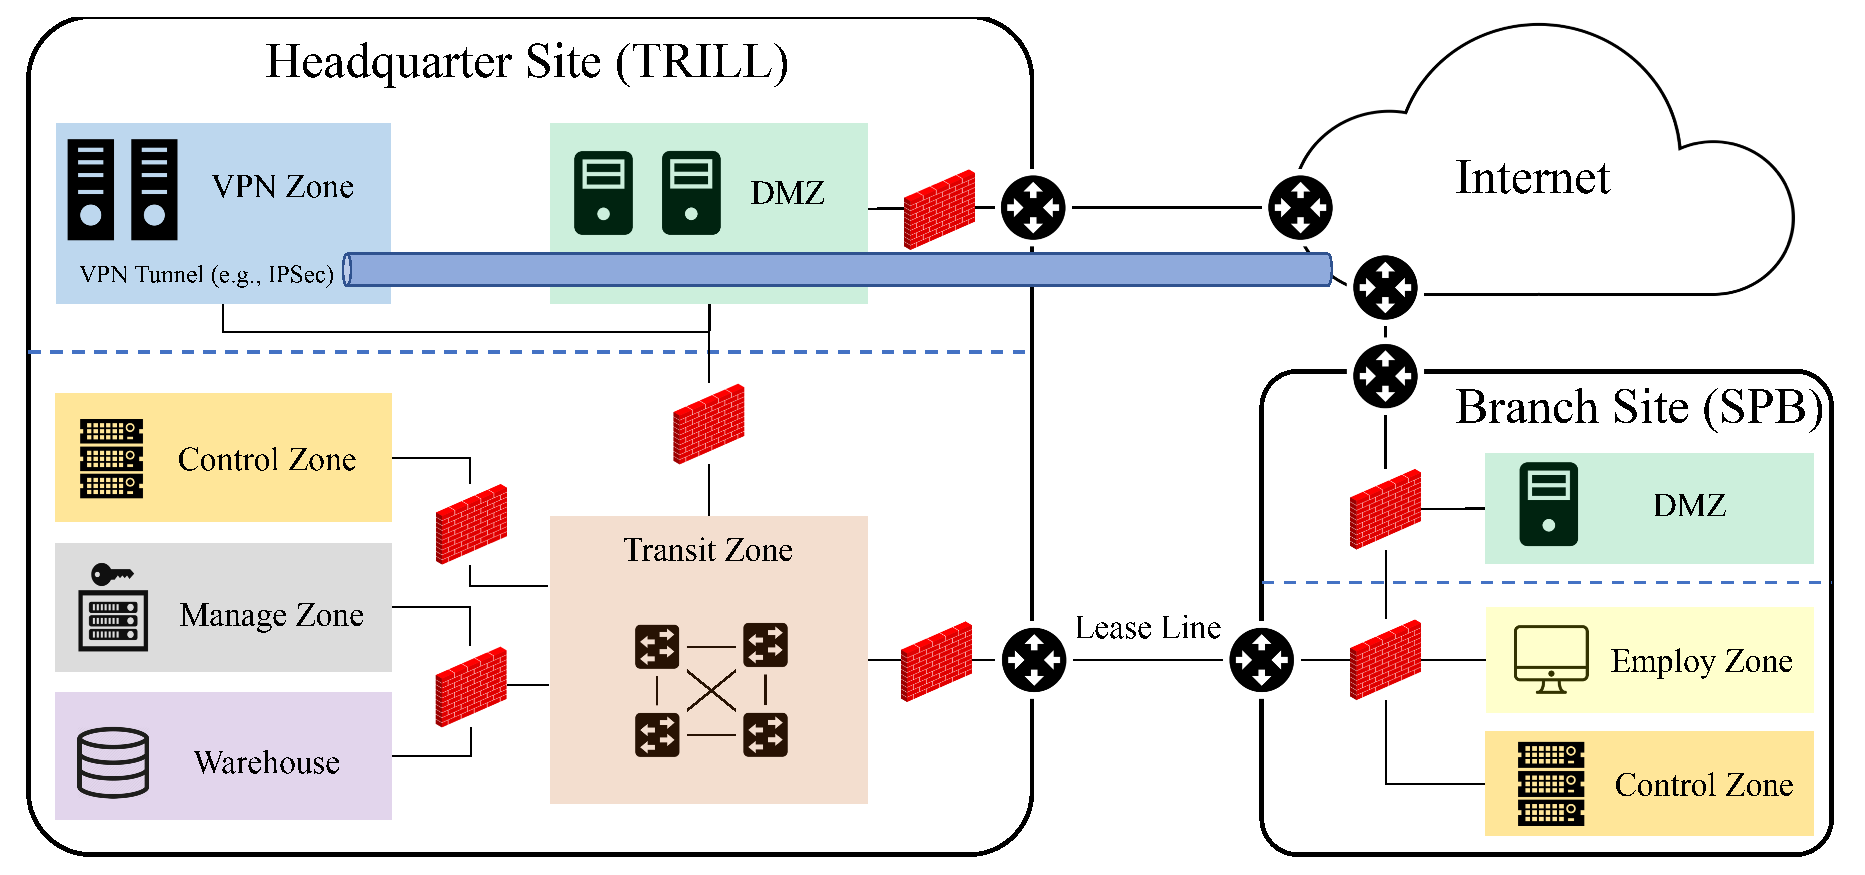
\includegraphics[width=.7\textwidth]{usecase.eps}
\end{center}
\caption{Network zoning use case for large enterprises. Network zones are 
realized with heavy use of security middleboxes (e.g., Firewalls).}
\label{fig:usecase}
\end{figure}

\paragraph{Inter-domain Zone Transfer}
% 1. to the same zone
% 2. to a different zone
To ensure that geographically distributed zones can securely communicate with each other, 
enterprises employ various networking technologies. The most common choice is connecting
two remote sites with a physical private line, (e.g., Layer 2 circuit). %or MPLS. 
% \ml{I would call an MPLS VPN a ``virtual private line'' as other traffic may flow over the same physical connections.} 
Enterprises 
can lease these lines from Internet service providers and make use of them to bridge local 
networks. However, purchasing private lines is costly and might come along 
with trust issues towards the service provider. 

An alternative is a virtual private 
network (VPN). A VPN uses cryptographic primitives to create a virtual tunnel between two 
local networks, preventing information leakage during transmission over the public Internet. 
While the VPN technology ensures data confidentiality, typically yet another layer of overlay 
protocols is required to achieve virtual separation of zones. The use of such overlay 
protocols, however, has the disadvantage that all interconnected sites need to deploy the same 
protocol since such protocols generally do not offer interoperability.

% \claude{While these techniques can be used to ensure confidentiality for data transmissions over an untrusted network, typically yet another layer of overlay protocols is required to achieve virtual separation of zones. The use of such overlay protocols, however, has the disadvantage that all interconnected sites need to deploy the same protocol since such protocols generally do not offer interoperability.}

% \claude{Where to put comparison of VPN point-to-point and \name Mondrian -> point to many}

\paragraph{Traffic from the Internet}
% 1. normal customer
% 2. authorised user (employ)
% 3. attacker
Traffic not originating from cooperative (trusted) networks can be classified 
into the following three types: i) public traffic, ii) authorized traffic, and iii) 
malicious traffic. The first case covers normal customers who access the enterprise's 
public services, e.g., Web servers. This traffic in general ends up at the demilitarized zone 
(DMZ) hosting only public services that require exposure to Internet. 
The second case refers to the traffic coming from temporarily authorized devices. For example,
a legitimate employee outside the enterprise's premises---working from home with a personal 
device---may get a temporal permit to access restricted zones via VPN. The last 
category comprises attack packets which are to be filtered by the security middleboxes in the frontline of defense.

% \begin{table}[t]
% % \caption{use case table. need to be merged with the fig_usecase}
% \label{tab:usecase}
% \centering
% \resizebox{0.48\textwidth}{!}{
% 	\begin{tabular}{*4{c}}
% 	\toprule
% 	& Between Zones & Through Transit Zone & Within Zone\\
% 	\midrule
% 	Inter-domain & \circled{1} $E_1 \leftrightarrow E_4$ 
% 	& \circled{2} $E_1 \leftrightarrow E_5$ & \circled{3} $E_1 \leftrightarrow E_2$\\
% 	Intra-domain & \circled{4} $E_5 \leftrightarrow E_6$ 
% 	& \circled{5} $E_3 \leftrightarrow E_4$ & \circled{6} $E_1 \leftrightarrow E_3$\\
% 	\bottomrule
% 	\end{tabular}
% }
% \end{table}

% \paragraph{Inter-domain Zone Transfer} % Case 1:
% \paragraph{Inter-domain Zone Transfer via Transit} % Case 2: 
% \paragraph{Inter-domain Communication within a Zone} % Case 3: 
% \paragraph{Local Zone Transfer} % Case 4: 
% \paragraph{Local Zone Transfer via Transit} % Case 5: 
% \paragraph{Local Communication within a Zone} % Case 6: 


\subsection{Challenges}
\label{ssec:challenges}

\paragraph{Secure Zone Transfer}
Transmitting security-sensitive data between zones in different physical locations (e.g., 
data center to branch site) over the public Internet poses a challenge. 
Security level information is lost in transit, requiring that the data is re-authenticated and 
filtered again on the receiving site even though source and destination could be part of the 
same logical zone.
Today's overlay protocols are often used to overcome the restriction of losing 
security level information in transit. This however introduces new challenges: difficulties 
in deployment per zone, computational overhead, and poor management scalability. 
% Driven by this, a light-weight zone transfer architecture is needed.

\paragraph{Interoperability}
Even if security-level information persists in transit, different zones might not be 
built on the same internal protocols (e.g., SPB~\cite{ieee2012spb} vs Trill~\cite{rfc6325}) 
which makes it difficult
for end systems in different zones to be able to seamlessly communicate with each other.
% A new architecture therefore must be able to understand various network protocols and 
% interpret them into a local language that all target networks can understand. This means 
% that the interpretation should preserve the properties of an original protocol, such as 
% % layer-2 routing decisions. 
% virtual segmentation.
% % A flexible design for the architecture to easily embed new protocols also should be considered.

\paragraph{Management Scalability}
In current local network zoning architectures, administration is being considered a tedious, 
time-consuming, and labor-intensive task. For example, simply adding a new zone might
require existing policies to be thoroughly reviewed, updated, and re-distributed
to the local network entities. The management complexity dramatically increases in a 
wide-area network (WAN) environment.
% For global orchestration across heterogeneous environments, a new architecture therefore
% must ensure management scalability. That is, network administrators should be able to easily extend 
% network zones in different physical locations and update policies that reflect these network
% changes, and be assured that no security loopholes were introduced.


% easily scale up resources 





% \subsection{Industrial Perspectives}

% % \paragraph{Large Enterprise Networks}
% % In order to protect information technology assets, large enterprise networks are partitioned into disjoint segments which group together assets with the same security requirements and policies. These groups are referred to as zones. Zones define the network boundaries and their defense requirements by stating the entities populating the zones, the entry points into the zone as well as how traffic is monitored and filtered at these entry points. Oftentimes, these zones are realized by a (virtualized) separation at layer 2 with firewalls at higher levels governing data transfers between zones.
% Traditionally, enterprises used to consider three security layers for their network 
% environment: intranet, extranet and opennet~\cite{ramasamy2011towards}. The opennet is
% the least trusted network (e.g., the Internet) which is inhospitable region where live 
% threats exist, while the intranet is the most trusted network hosting business-critical 
% systems and sensitive information. Since the intranet has rigorous access controls to 
% protect the information assets from an exposure, enterprises put another security layer 
% (extranet) in between, that only exposes public services to opennet and thus reduces 
% attack surfaces. 
% As enterprises have recently witnessed extreme changes in network environment such as
% diverse demands from customers, partners and employees accessing their network with
% variety of devices, the enterprises employ more sophisticated network security 
% segmentation\cite{obregon2015infrastructure}, called security zones.
% Security zones constitute the logical grouping of one or more subnets that share the
% same security requirements and policies. 
% % Since security zoning is the foundation of 
% % network isolation criteria that must be upheld for secure business environements, 
% % the zone classification of information assets requires 

% Each security zone is identified with different level of trust, and every pair of zones 
% are defined with a namely trusted-untrusted relationship. 
% To realize the unidirectional trust model, firewalls are considered as the most viable
% technologies and widely used in the current practice. However, operating firewalls in 
% large enterprises is often challenging to network operators and security architects. The 
% access control for the security zones might be dynamic, and thus its requires a complex 
% management scheme to accommodate a myriad set of policies. While there are advanced 
% technologies such as virtual firewall~\cite{deng2015vnguard,bakker2016network} and Unified
% Threat Management (UTM)~\cite{qi2007towards}, that are newly designed for enforcement of 
% access control polices in extremely dynamic networks, security zone management and modeling 
% still remains to be evolved~\cite{ramasamy2011towards,gontarczyk2015blueprint}.

% Bridging geographically distant security zones can also be challenging. Oftentimes,
% security zones are created not only for security purpose but also because of geographical
% factors. Given that the security zones in distance should exchange information over
% public network (opennet as aforementioned), there might be a potential risk that the
% communication may expose security-sensitive information during transit. To mitigate
% such a threat, network operators leverage additional security control/mechanisms (e.g.,
% IPSec~\cite{rfc4301} and SSL VPN~\cite{sun2011advantages}) which ensure confidentiality
% and integrity of the transmission over the untrusted network by encrypting the data with
% securely shared cryptographic keys. Nonetheless, the technologies might bring new challenges
% such as management scalability~\cite{felsch2018dangers} and compatibility to the secure 
% isolation~\cite{liu2008collaborative}.

% % \paragraph{Cloud Computing (LaaS, PaaS, SaaS)}
% The cloud computing environment is a good representative example that depicts such practical 
% challenges. Cloud-based service providers operate large multi-tenant data centers which 
% have to scale to customers needs. To achieve this scalability while at the same time staying
% cost efficient cloud providers make heavy use of virtualization techniques. This environment 
% challenges operators with providing secure segmentation between tenants as multiple tenants 
% are using the same physical machines and network. In addition, given that the cloud 
% environments comprise geographically distributed data centers, providing secure communication 
% channels between security zones while upholding a constant view of the security policies
% under the dynamic zone migration is another hill to climb. Now, we derive main challenges 
% we confront in this research with case study.
% % Legal requirements need to be respected. Furthermore, an optimal solution needs to be highly 
% % flexible as the number of assigned resources for a given customer can change frequently.



% % \paragraph{Edge Computing}
% % With the rise of mobile devices and Internet of Things (IoT) new types of data intensive, time sensitive applications are emerging. (e.g. VR/AR) However, since these devices are also required to be low power they cannot do these heavy computations themselves. Cloud computing can be used to offload the work to centralized data centers. However, this causes new challenges. Often, the latency between devices and the cloud is too high and therefore not well suited for real-time applications. Additionally, a large number of devices means that a centralized infrastructure can get saturated by big traffic flows. One widely used solution to this problem is Edge Computing which puts nodes handling the computation close to end devices.
 % Background Theory
\chapter{Diagnosing Overthinking}
\label{overthinking}

This chapter presents our framework for identifying and analyzing overthinking behavior in Large Reasoning Models (LRMs). We begin by defining the Reasoning-Action Dilemma that leads to overthinking, then describe the manifestations of this behavior, and finally present our methodology for quantifying it. Through our analysis of 3,908 trajectories, we demonstrate that overthinking represents a significant challenge in agentic environments, particularly affecting models specifically trained for reasoning tasks.

\section{The Reasoning-Action Dilemma}
\label{sec:dilemma_detailed}

We observe that, in agentic decision-making tasks, LRMs constantly face the \emph{Reasoning–Action Dilemma}. This fundamental trade-off requires models to balance two competing approaches: direct interaction with the environment through action execution and feedback collection, and internal reasoning where models simulate hypothetical outcomes before committing to actions. This dilemma is particularly challenging because both approaches have their merits—environmental interaction provides ground truth but can be costly or risky, while internal reasoning allows for safe exploration but may diverge from reality.

Ideally, an LRM should balance reasoning and action by using internal simulation to refine its choices while leveraging real-world feedback to correct errors. For instance, when debugging a failing test case, a well-balanced model would hypothesize potential issues yet still execute the test opportunely to collect concrete failure signals. This balance is particularly critical in software engineering tasks, where models must understand complex codebases, reason about potential fixes, and validate their solutions through testing.

Unfortunately, achieving this balance is inherently challenging. In such settings, feedback is sparse, compelling LRMs to rely heavily on internal simulation to make the most out of every iteration. However, prior research has demonstrated that LRMs exhibit significant vulnerability to knowledge insufficiency, where gaps in understanding can cascade into compounding errors throughout the reasoning process \cite{li2025searcho1agenticsearchenhancedlarge, zhong2024evaluationopenaio1opportunities, LingFLHLMS23, chia2024reasoningpathsoptimizationlearning}. This challenge is exacerbated by LRMs' sensitivity to prompt modifications \cite{openai_learning_to_reason_2024, deepseekai2025deepseekr1incentivizingreasoningcapability}, which can disrupt their ability to maintain and process contextual information. These limitations become especially critical in agentic scenarios, where models must simultaneously gather, retain, and act upon new information \cite{zhang2024agenticinformationretrieval, yang2024sweagentagentcomputerinterfacesenable}. Consequently, excessive simulation without sufficient external information can ultimately lead to failure. The situation is especially difficult for environments with limited interaction opportunities.

\section{Manifestations of Overthinking}
\label{sec:manifestations_detailed}

Our investigation into impaired decision-making in AI agents draws from a detailed analysis of agent-environment interactions. These interactions are recorded in what we term trajectories - comprehensive logs that capture the complete sequence of agent actions, environment responses, and (where available) the agent's reasoning process. As outlined in \cref{evaluation_framework}, we systematically analyzed these trajectories to understand patterns of \textbf{overthinking}.

While most trajectories include the agent's explicit reasoning process, those from the o1 family exclude these reasoning tokens \cite{openai_learning_to_reason_2024}. This limitation led us to focus our analysis on observable behaviors, which are the concrete actions agents take in response to environmental challenges.

Through this analysis, we identified three distinct patterns of \textbf{overthinking}, as illustrated in \cref{fig:manifestations}:

\subsection{Analysis Paralysis}
When faced with challenges, LRMs tend to shift their focus from immediate actions to elaborate future planning. They generate increasingly complex action sequences but struggle to execute them systematically. Rather than addressing immediate errors, they construct intricate plans that often remain unexecuted, leading to a cycle of planning without progress. This behavior is particularly evident in software engineering tasks, where models may spend excessive time analyzing potential code changes without actually implementing and testing them.

\subsection{Rogue Actions}
We observe cases where agents deliberately try to bypass environmental exploration by generating chains of interdependent actions in a single step. Despite their prior demonstrated awareness of step-by-step interaction requirements, models proceed to construct elaborate action sequences that presume the success of each preceding step, effectively substituting real environmental feedback with internal simulation. This behavior often manifests as attempts to execute multiple file modifications or system commands simultaneously, without waiting for confirmation of each step's success.

\subsection{Premature Disengagement}
LRMs sometimes terminate tasks based solely on their internal simulation of the problem space, either through direct abandonment or by delegating hypothetical action sequences. This illustrates how overreliance on internal reasoning can lead to decisions without environmental validation. For example, a model might declare a bug fixed based on its analysis of the code changes, without actually running the tests to verify the fix works as intended.

\section{Quantifying Overthinking}
\label{sec:quantifying}

To systematically study overthinking in LRMs, we developed a comprehensive evaluation framework that combines automated analysis with human validation. Our approach focuses on quantifying the degree to which models favor internal reasoning over environmental interaction, allowing us to measure the impact of overthinking on model performance and identify potential mitigation strategies. Through this framework, we analyzed 3,908 trajectories across 19 different models, revealing significant patterns in how overthinking manifests and affects model behavior in agentic environments.

\subsection{Overthinking Score}
To quantify overthinking behavior, we developed a systematic scoring method using an LLM-based evaluator. This evaluator analyzes model trajectories for the previously described patterns and assigns a score from 0 to 10, with higher scores indicating more severe overthinking behavior. Each score includes a detailed justification explaining which patterns were identified and their severity. The complete evaluation prompt and scoring criteria can be found in \cref{apx:prompt_overthinking}.

Our analysis reveals two distinct patterns in overthinking behavior. First, regression analysis demonstrates a significant negative correlation between overthinking and issue resolution rates for both reasoning and non-reasoning models (\cref{fig:figure1}), with the latter showing a steeper decline in performance as overthinking increases. Second, a direct comparison reveals that reasoning models consistently exhibit higher overthinking scores—nearly three times higher than non-reasoning models—with this difference being statistically significant as shown in \cref{tab:overthinking_scores}.

\subsection{Validation Methodology}
To validate our LLM-based evaluator, we conducted an independent assessment where four expert annotators manually scored 20 randomly selected model traces. The Spearman rank correlation ($p = 0.800$) between human experts and our automated scoring system demonstrated a strong monotonic relationship, as shown in \cref{fig:human_eval}. This non-parametric correlation measure confirms the reliability of our overthinking measurement methodology.

\subsection{Impact on Model Performance}
Statistical analysis reveals that higher overthinking scores correlate with decreased performance across all models. This correlation is particularly strong for reasoning models, which exhibit consistently higher overthinking tendencies, suggesting that excessive reliance on internal simulation impairs task performance. As illustrated in \cref{fig:figure1}, model nomenclature such as "FC" (indicating native function calling capability), "DS" (representing DeepSeek models), and suffixes o1\_high and o1\_low denoting models with reasoning effort set to high and low respectively, all show this consistent pattern.

\subsection{Practical Implications}
Our findings demonstrate that simple efforts to mitigate overthinking can yield substantial benefits. By generating two candidate solutions using o1 with low reasoning effort and selecting the one with lower overthinking score, we not only improved issue resolution from 21\% to 26.3\% on SWE Bench Verified tasks (\cref{fig:figure2}), but also nearly matched the performance of high-reasoning configurations while \textbf{reducing computational costs by approximately 43\%}. This demonstrates that simple overthinking mitigation strategies can dramatically improve the efficiency of LRMs in real-world applications.

\section{Evaluation Framework}
\label{sec:eval_framework}

Our evaluation framework consists of several key components designed to systematically analyze overthinking behavior in LRMs. We employ SWE Bench Verified \cite{jimenez2024swebenchlanguagemodelsresolve, swebench_verified} as our benchmark, using the CodeAct agent scaffolding \cite{wang2024executablecodeactionselicit} within the OpenHands framework \cite{wang2024openhandsopenplatformai}. This setup creates a controlled environment where models must balance information gathering with reasoning chains while maintaining context across multiple interactions as illustrated in \autoref{fig:figure3}.

\subsection{Models Evaluated}
To comprehensively study the phenomenon and influence of overthinking, we evaluated 19 models selected to represent diverse characteristics across the current LLM landscape. Our selection spans both reasoning-optimized models and general-purpose language models to understand how specialized reasoning training affects overthinking tendencies. We included both proprietary models (such as OpenAI's o1 and Claude Sonnet 3.5) and open-source alternatives (like DeepSeek-R1 and Qwen2.5) to ensure our findings generalize across different development approaches. The models range in size from relatively small (1.5B-14B parameters) to large-scale architectures (32B-671B parameters), allowing us to investigate how model scale influences overthinking behavior. Additionally, we compared models with native function calling capabilities (such as OpenAI o1 and GPT-4o) against those without, to understand how explicit tool-use training affects environmental interaction patterns.

\subsection{Trajectory Analysis}
Our analysis centers on comprehensive interaction logs that we term trajectories. Each trajectory captures the complete temporal sequence of model actions, including precise timing information, along with the corresponding environmental responses. Where available, we also record the model's internal reasoning process, though this is notably absent in some models like the o1 family. These logs culminate in clear success or failure indicators for each task attempt, providing objective metrics for performance evaluation.

Through our analysis of \textbf{3,908 trajectories}, we have created a comprehensive open-source dataset to advance research in balancing reasoning and action in agentic environments. Each trajectory is accompanied by its overthinking score and detailed justification, enabling future researchers to build upon our findings and develop improved strategies for managing the reasoning-action trade-off.

\subsection{Pattern Recognition}
Our framework employs a systematic approach to identify key behavioral patterns indicative of overthinking. We focus particularly on extended reasoning chains that lack corresponding actions, as these often signal a model's excessive reliance on internal simulation. We also track instances where models attempt to generate multiple actions in a single turn, bypassing the intended step-by-step interaction process. Additionally, we monitor for premature task termination and cases where models disregard environmental feedback, both of which suggest an overreliance on internal world models rather than real-world interaction.

These patterns are evaluated within the context of software engineering tasks, where we can leverage automated test suites and code validation tools to objectively measure task completion. This approach ensures our pattern recognition is grounded in concrete, measurable outcomes rather than subjective assessments.

\subsection{Statistical Validation}
Our statistical analysis reveals three key findings about overthinking in language models: its relationship with performance in SWE-bench, its non-equal prevalence across model types, and its practical implications for model selection. We employ rigorous statistical methods to ensure the reliability of our findings.

Regression analysis demonstrates a significant negative correlation between overthinking and issue resolution rates for both reasoning and non-reasoning models. Non-reasoning models show a steeper decline in performance as overthinking increases, with a beta coefficient of -25.802 compared to -11.476 for reasoning models. Both relationships are statistically significant (p = 0.031 and p = 0.006 respectively).

A direct comparison reveals that reasoning models consistently exhibit higher overthinking scores—nearly three times higher than non-reasoning models. Reasoning models average 2.320 ± 1.120 on our overthinking scale, while non-reasoning models score 0.865 ± 0.432. This difference is statistically significant (p = 0.019), suggesting a systematic tendency toward overthinking in reasoning-optimized models.

To validate our automated scoring system, we conducted an independent assessment with four expert annotators who manually scored 20 randomly selected model traces. The Spearman rank correlation (p = 0.800) between human experts and our automated system demonstrates a strong monotonic relationship, confirming the reliability of our measurement methodology.

The complete analytical framework and results are presented in \cref{evaluation_framework}. The tools used for the statistical analysis can be found in \cref{stat_framework}.

\section{Implementation Details}
\label{sec:implementation}

\subsection{LLM-as-Judge System}
Following the LLM-as-a-judge methodology \cite{zheng2023judgingllmasajudgemtbenchchatbot}, we developed a specialized evaluation system using Claude Sonnet 3.5 as our judge model. The system is configured for maximum reliability and transparency, with temperature set to 0 to ensure deterministic scoring across evaluations. We leverage Claude's 200k token context window to process complete trajectories alongside detailed evaluation criteria, and enforce a structured output format to maintain consistency across assessments. Each evaluation must include detailed justifications, enabling thorough review and validation of the scoring process.

Claude Sonnet 3.5 was selected specifically for its extensive context window and proven reliability in complex evaluation tasks. To prevent bias, we deliberately withhold final issue resolution outcomes from the evaluator, ensuring that overthinking assessments are based purely on behavioral patterns rather than task success. This approach maintains the independence of our overthinking metrics from performance measures, allowing us to analyze their relationship without circular dependencies.

\subsection{Scoring Criteria}
Our scoring system implements a multi-dimensional evaluation approach that considers several key aspects of model behavior. At its core, we assess how well models balance their reasoning processes with concrete actions, looking for evidence of effective decision-making that combines thoughtful analysis with practical implementation. We evaluate the model's ability to appropriately incorporate environmental feedback into its decision-making process, particularly focusing on how it adapts its approach based on system responses. The efficiency of the problem-solving approach is also considered, examining whether models take unnecessarily complex paths or maintain a focused, goal-oriented strategy. Finally, we track the completion of necessary validation steps, ensuring that models don't skip crucial verification processes in their rush to propose solutions.

\subsection{Model Size and Overthinking}
Our initial hypothesis posited that smaller LRMs would struggle more with environmental comprehension, leading them to rely heavily on internal reasoning chains and thus exhibit increased overthinking behavior. To test this hypothesis, we analyzed two model families across four size variants (32B, 14B, 7B, and 1.5B): the non-reasoning Qwen2.5-Instruct and the reasoning R1-Distill-Qwen.

Our analysis revealed a strong negative correlation between model size and overthinking scores: larger models demonstrated less tendency to overthink, as shown in \cref{figure5}. The distinction between reasoning and non-reasoning models becomes particularly pronounced at smaller scales. R1 models exhibit significantly higher overthinking scores (5.157 ± 2.292) compared to their Qwen2.5 counterparts (1.771 ± 0.463), with this gap widening as model size decreases. This difference is statistically significant (t = 2.508, p = 0.046).

\subsection{Token Usage Analysis}
We investigated the relationship between token consumption and overthinking behavior in the o1 model. We conducted experiments by manipulating the model's reasoning effort parameter between high and low settings, which influences the number of reasoning tokens used \cite{openai_chat_api}. Our analysis revealed an unexpected pattern: in agent-based scenarios, o1 models with low reasoning effort demonstrated 35\% higher overthinking scores compared to their high-effort counterparts. As shown in \cref{tab:o1_model_comparison}, the difference in averaged overthinking scores between the two configurations is statistically significant, suggesting that increased token allocation might paradoxically reduce overthinking in agentic contexts.

\subsection{Function Calling Impact}
Our experimental analysis compared O1 model configurations with high reasoning effort, evaluating performance both with and without native function calling (FC) capabilities. The integration of FC capabilities yielded substantial improvements across multiple metrics. Most notably, we observed a dramatic increase in performance score from 29.1\% to 47.7\%, accompanied by a significant reduction in average overthinking score from 2.47 to 0.56. These improvements suggest that native function calling capabilities help models maintain a more balanced approach to environmental interaction.

However, benchmarking against BCFL \cite{berkeley-function-calling-leaderboard} reveals a more nuanced pattern. In multi-turn environments, the performance differential between FC and non-FC implementations of O1 shows a more modest improvement from 36\% to 41\%. This comparatively smaller enhancement suggests that FC implementation alone cannot fully account for the dramatic performance improvements observed in our primary experiments, indicating that other factors may play significant roles in reducing overthinking behavior.

OpenAI has demonstrated that reasoning models exhibit a disproportionate increase in computational costs relative to their performance gains \cite{arcprize2024oai}. Our experiments with SWE-bench Verified dataset confirm this observation: o1 with high reasoning effort achieves a 29.1\% resolution rate at \$1,400, while the low reasoning variant reaches 21.0\% at \$400—a 3.5x cost difference for an 8.1 percentage point improvement in performance.

To address this efficiency gap, we developed an alternative approach: running the low-reasoning variant twice and selecting traces with minimal overthinking scores. This method achieved a 26.3\% resolution rate while consuming only 57\% of the high-reasoning configuration's cost. Our findings suggest that monitoring and controlling overthinking behavior could be a cost-effective strategy for optimizing model performance in real-world applications.

\section{Limitations and Considerations}
\label{sec:limitations}

While our framework provides valuable insights into overthinking behavior, it has several limitations that inform our ongoing research directions:

\subsection{Technical Limitations}
Our framework, while effective, faces several significant technical constraints. A primary challenge stems from limited access to internal reasoning processes, particularly in models like o1 that exclude reasoning tokens \cite{openai_learning_to_reason_2024}. This limitation forces us to rely primarily on observable behaviors, potentially obscuring important aspects of the overthinking process that manifest in internal model states.

The use of LLM-based evaluation, while showing strong correlation with human judgments, introduces its own set of challenges. While Claude Sonnet 3.5 has proven reliable as an evaluator, its use may introduce systematic biases in overthinking detection that could affect our analysis. This concern is particularly relevant given the complex nature of the behaviors we're trying to quantify.

Resource constraints also pose significant challenges to our approach. Processing and analyzing our dataset of 3,908 trajectories requires substantial computational resources, particularly when evaluating models with high reasoning effort settings. This computational burden becomes especially pronounced when dealing with larger language models or more complex interaction patterns. As we look to expand our analysis to larger datasets or more intricate environmental interactions, these scalability challenges may become increasingly significant.

\subsection{Methodological Considerations}
Our methodology, while systematic, faces several important limitations in its current form. While we've identified three main patterns of overthinking, the complexity of model behavior suggests there may be additional manifestations that our current framework doesn't capture. This potential incompleteness in our pattern identification could affect our ability to fully characterize overthinking behavior in different contexts.

The human validation process presents another significant challenge. Validating overthinking scores requires substantial expert time and attention, with each trajectory requiring careful analysis to ensure accurate assessment. This intensive validation process may not scale well to larger studies, potentially limiting our ability to expand the scope of our analysis.

Domain specificity also presents a methodological concern. Our findings are primarily based on software engineering tasks using SWE Bench Verified, and while these provide a rich environment for studying model behavior, the patterns and implications we've identified may not generalize uniformly to other domains. Different task environments might elicit different manifestations of overthinking, requiring additional validation and potentially different evaluation criteria.

The relationship between model scale and overthinking behavior adds another layer of complexity to our methodology. Our analysis of DeepSeek-R1-671B, which revealed overthinking scores comparable to DeepSeek-V3-671B, suggests that model scale and training methodology interact in ways that are not yet fully understood. This observation highlights the need for more nuanced evaluation approaches that can account for these complex interactions.

\subsection{Future Research Directions}
Our analysis suggests two promising approaches to mitigate overthinking in LRMs. First, the success of function-calling architectures hints at the importance of explicit interaction training, though our BCFL benchmarking indicates this alone isn't sufficient for optimal performance. Second, the effectiveness of limited reinforcement learning in DeepSeek-R1-671B points to the crucial role of training methodology in controlling overthinking tendencies.

These findings raise several critical questions for future research. A primary concern is how these approaches might generalize across different domains, as the effectiveness of mitigation strategies may vary significantly depending on the specific requirements and constraints of each application area. We must also consider how to optimize these approaches for environments where environmental interaction carries varying costs, balancing the benefits of active exploration against operational constraints. Additionally, the role of model scale in overthinking behavior requires further investigation, as our results suggest complex interactions between model size, architecture, and overthinking tendencies.

Understanding these dynamics could help develop more robust solutions that prevent, rather than just mitigate, overthinking behaviors in large reasoning models. To facilitate further research in this direction, we release our evaluation framework and dataset of 3,908 trajectories, enabling the broader research community to build upon these findings across different environments and architectures.
 % Diagnosing Overthinking
\chapter{Evaluation}
\label{eval}

To assess the impact of overthinking in Large Reasoning Models, we analyze their performance in agentic environments using SWE-Bench Verified, comparing reasoning models with their non-reasoning counterparts. Our study aims to answer the following research questions:
\begin{itemize}
    \item RQ1: Does overthinking affect performance?
    \item RQ2: Does its impact affect all models equally?
    \item RQ3: How to potentially mitigate overthinking?
\end{itemize}

\section{Experimental Setup}
\label{sec:setup}

\subsection{Models Evaluated}
To comprehensively study the phenomenon and influence of overthinking, we consider 19 models across multiple dimensions, including reasoning capabilities, model openness (proprietary vs. open-source), model size, and function calling support. We evaluate both reasoning-optimized models as well as general-purpose language models. Our evaluation spans proprietary models (e.g., OpenAI o1, Claude Sonnet 3.5)~\cite{openai_learning_to_reason_2024,anthropic_claude_3_5} and open-source alternatives (e.g., DeepSeek-R1, Qwen2.5) \cite{qwen2, qwen2.5, deepseekai2025deepseekr1incentivizingreasoningcapability} to ensure broad coverage.

We also analyze models of varying scale, ranging from small (1.5B-14B) to large-scale models (32B-671B parameters) \cite{deepseek_reasoning_model}, to investigate whether model size influences overthinking tendencies. Additionally, we distinguish between models that natively support function calling (e.g., OpenAI o1, GPT-4o) \cite{openai_function_calling, openai_gpt4o_2024, openai_gpt4o_mini, openai_o1} and those that do not, which allows us to assess whether explicit function calling capabilities reduce overthinking compared to models that rely on prompt-based learning of tool usage. Further details on the models studied can be found in the~\autoref{apx:models},~\autoref{tab:model_comparison}.

\subsection{Scaffoldings}
To enable tool use, we adopt CodeAct, an open-source single-agent scaffolding built within the OpenHands framework~\cite{openhands}, as models alone cannot directly execute code or edit files~\cite{qwq-32b-preview, openai_o1_mini, openai_o1_system_card_2024, deepseekai2025deepseekr1incentivizingreasoningcapability, sky_t1_2025}. Scaffolding provides a structured execution environment, allowing models to interact with SWE-bench in a controlled and consistent manner. We choose the single-agent approach as it maintains a unified reasoning process, ensuring full context retention throughout execution.

In contrast, multi-agent scaffolds distribute tasks across multiple specialized agents that share an underlying model but operate with distinct prompts and action spaces~\cite{chen2024coderissueresolvingmultiagent,xia2024agentlessdemystifyingllmbasedsoftware, phan2024hyperagentgeneralistsoftwareengineering, allhands_single_agent_systems} which can introduce structural rigidity and lead to information loss during inter-agent communication~\cite{allhands_single_agent_systems}. Similarly, since our goal is to evaluate tool use and in-context memory, we avoid OpenAI's Agentless approach~\cite{openai_o1_system_card_2024, xia2024agentlessdemystifyingllmbasedsoftware}, which follows a fixed three-step process (localization, repair, patch validation) without allowing adaptive decision-making. Therefore, we can ensure all models are evaluated in a standardized, interactive environment.

\section{Overthinking Score Calculation}
\label{sec:score_calc}

We devise an LLM-based evaluation framework with a carefully designed prompt to systematically assess overthinking behaviors. This evaluator is instructed to recognize overthinking patterns, as described in~\autoref{sec:manifestations}, within model trajectories in agentic scenarios. Based on the identified patterns, the evaluator assigns an overthinking score on a scale from 0 to 10 and provides a detailed justification for the assigned score.

To ensure reliability and consistency, we employ Claude Sonnet 3.5 as the evaluation model and configure it with a temperature of 0 to enforce deterministic scoring, following the LLM-as-a-judge methodology~\cite{zheng2023judgingllmasajudgemtbenchchatbot}. Claude Sonnet 3.5 was selected for its 200k-token context window, allowing it to process complete trajectories alongside the evaluation criteria.

Notably, the evaluator does not have access to the final issue resolution outcome, ensuring that the overthinking assessment remains independent of task success and thereby eliminating potential biases. The complete evaluation prompt and scoring criteria can be found in \cref{apx:prompt_overthinking}. % Evaluation
\chapter{Results}
\label{results}

We generate and evaluate \textbf{3908 trajectories} using our evaluation methodology across all models. We make publicly available every trajectory alongside their corresponding overthinking score and the reasoning behind this score.

Our analysis reveals three key findings about overthinking in language models: its relationship with performance in SWE-bench, its non-equal prevalence across model types, and its practical implications for model selection. We observed that overthinking consistently impacts performance across all evaluated models, with reasoning-optimized models showing higher overthinking tendencies than general-purpose ones.

\section{Overthinking and Performance}
\label{sec:perf}

We anticipated that overthinking should impact performance as if models rely too heavily on their internal reasoning chain, there is a high likelihood that they will propose fixes based on inaccurate claims.

We observed a strong negative correlation between overthinking and performance on SWE-bench, as illustrated in \cref{fig:figure1}. Both reasoning and non-reasoning models show decreased performance as overthinking increases, though with notably different patterns.

\section{Overthinking and Model Type}
\label{sec:model_type}

We make three key observations with regards to overthinking in reasoning and non-reasoning models:

\subsection{Non-reasoning Models Can Overthink}
This observation can be explained by the presence of reasoning capabilities in non-reasoning models which could lead to overthinking. Recent studies show that non-reasoning models could have reasoning capabilities \cite{wei2023chainofthoughtpromptingelicitsreasoning, yao2023treethoughtsdeliberateproblem, chen2023program, kojima2023largelanguagemodelszeroshot}.

\subsection{Higher Overthinking in Reasoning Models}
Reasoning models significantly have higher overthinking scores compared to non-reasoning models, as shown in \cref{tab:overthinking_scores}. Since these models are specifically trained to reason and generate extended chains of thought by simulating environment interaction, they are more likely to suffer from manifestations of overthinking.

\subsection{Severe Impact on Non-reasoning Models}
Non-reasoning models that overthink suffer from severe degradation in issue resolution, as evidenced by the beta coefficients shown in \cref{tab:regression_results}. Lower beta coefficients indicate higher impact of overthinking on performance. We suspect that since non-reasoning models are not trained for reasoning, they are not capable of handling reasoning chains effectively, thus showing worse results.

\begin{table}[ht]
\centering
\begin{tabular}{lcccc}
\toprule
\textbf{Model} & \boldmath{$\beta_1$} & \boldmath{$R^2$} & \textbf{p-value} \\
\midrule
Reasoning      & -11.476 & 0.808 & 0.006 \\
Non-Reasoning  & -25.802 & 0.727 & 0.031 \\
\bottomrule
\end{tabular}
\caption{Regression Results for Reasoning and Non-Reasoning Models}
\label{tab:regression_results}
\end{table}

\begin{table}[ht]
\centering
\begin{tabular}{lc}
\toprule
\textbf{Measure} & \textbf{Value} \\
\midrule
Reasoning Models       & 2.320 $\pm$ 1.120 \\
Non-Reasoning Models   & 0.865 $\pm$ 0.432 \\
\midrule
T-test p-value         & 0.019 \\
\bottomrule
\end{tabular}
\caption{Average Overthinking Scores for Reasoning and Non-Reasoning Models}
\label{tab:overthinking_scores}
\end{table}

\section{Overthinking and Model Size}
\label{sec:model_size}

We analyzed two model families across four size variants (32B, 14B, 7B, and 1.5B): the non-reasoning Qwen2.5-Instruct \cite{qwen2,qwen2.5} and the reasoning R1-Distill-Qwen \cite{deepseekai2025deepseekr1incentivizingreasoningcapability}. Our analysis revealed two key patterns:

\begin{enumerate}
    \item Larger models demonstrate less tendency to overthink
    \item The gap in overthinking scores between reasoning and non-reasoning models widens at smaller scales
\end{enumerate}

As detailed in \cref{tab:overthinking_comparison}, R1 models exhibit significantly higher overthinking scores compared to their Qwen2.5 counterparts, with this gap widening as model size decreases.

\begin{table}[ht]
\centering
\begin{tabular}{lccc}
\bottomrule
\textbf{Measure} & \textbf{Value} \\
\midrule
DS-R1 Family        & 5.157 $\pm$ 2.292 \\
Qwen2.5 Family      & 1.771 $\pm$ 0.463 \\
\midrule
T-test statistic     & 2.508 \\
T-test p-value       & 0.046 \\
\bottomrule
\end{tabular}
\caption{Overthinking Score Comparison for R1 and Qwen2.5}
\label{tab:overthinking_comparison}
\end{table}

\section{Overthinking and Token Usage}
\label{sec:token_usage}

We investigated the relationship between token consumption and overthinking behavior in the o1 model by manipulating the model's reasoning effort parameter between high and low settings. Our analysis revealed that o1 models with low reasoning effort demonstrate 35\% higher overthinking scores compared to their high-effort counterparts.

As shown in \cref{tab:o1_model_comparison}, the difference in averaged overthinking scores between the two configurations is statistically significant, suggesting that increased token allocation might reduce overthinking in agentic contexts.

\begin{table}[ht]
\centering
\begin{tabular}{lc}
\toprule
\textbf{Measure} & \textbf{Value} \\
\midrule
O1 Low        & 3.327 $\pm$ 4.539 \\
O1 High       & 2.467 $\pm$ 4.123 \\
\midrule
T-test p-value & 0.050 \\
\bottomrule
\end{tabular}
\caption{Comparison of o1 Models with Different Reasoning Efforts}
\label{tab:o1_model_comparison}
\end{table}

\section{Overthinking and Context Window}
\label{sec:context_window}

When comparing models of similar size but different context windows—such as DS-R1-32B versus QwQ and GPT-4o-mini versus SkyT1—we found no consistent relationship between context window size and overthinking tendencies. These observations suggest that context window size may not be a primary factor in determining a model's propensity for overthinking.

\section{Practical Implications}
\label{sec:implications}

OpenAI has demonstrated that reasoning models exhibit a disproportionate increase in computational costs relative to their performance gains \cite{arcprize2024oai}. Our experiments with SWE-bench Verified dataset confirm this observation: o1 with high reasoning effort achieves a 29.1\% resolution rate at \$1,400, while the low reasoning variant reaches 21.0\% at \$400—a 3.5x cost difference for an 8.1 percentage point improvement in performance.

To address this efficiency gap, we developed an alternative approach: running the low-reasoning variant twice and selecting traces with minimal overthinking scores. This method achieved a \textit{26.3\% resolution rate while consuming only 57\% of the high-reasoning configuration's cost}, as shown in \cref{fig:figure2}. Our findings suggest that monitoring and controlling overthinking behavior could be a cost-effective strategy for optimizing model performance in real-world applications. % Results
\chapter{Discussion}
\label{discussion}

\section{Native Function Calling Impact}
\label{sec:function_calling}

Our experimental analysis compared O1 model configurations with high reasoning effort, evaluating performance both with and without native function calling (FC) capabilities. The integration of FC capabilities yielded substantial improvements, increasing the performance score from 29.1\% to 47.7\%, while simultaneously reducing the average overthinking score from 2.47 to 0.56 -- effectively mitigating the overthinking phenomenon.

However, benchmarking against BCFL \cite{berkeley-function-calling-leaderboard} reveals a more nuanced pattern, where the performance differential between FC and non-FC implementations of O1 in multi-turn environments shows a modest improvement from 36\% to 41\%. This comparatively smaller enhancement suggests that FC implementation alone cannot fully account for the dramatic performance improvements observed in our primary experiments.

\section{The Case of DeepSeek-R1-671B}
\label{sec:deepseek}

Our analysis of DeepSeek-R1-671B (DS-R1) revealed overthinking scores comparable to those of DeepSeek-V3-671B. This similarity in overthinking behavior may be attributed to DS-R1's training methodology, which did not incorporate extensive reinforcement learning for software engineering tasks. While DS-R1 maintains performance levels similar to DeepSeek-V3 on software engineering benchmarks \cite{deepseekai2025deepseekr1incentivizingreasoningcapability}, our findings suggest that the combination of limited RL training and substantial model scale (671B parameters) contributed to its controlled overthinking behavior.

\section{How to Fix Overthinking}
\label{sec:solutions}

While our algorithmic interventions demonstrate immediate practical benefits, they primarily address the symptoms rather than the root causes of overthinking. Our analysis suggests that more fundamental solutions might emerge from understanding how models learn to balance reasoning and environmental interaction. The success of function-calling architectures hints at the importance of explicit interaction training, while the effectiveness of limited reinforcement learning points to the role of training methodology.

These insights open important questions for future research:
\begin{itemize}
    \item How do these approaches generalize across different domains?
    \item How can we optimize for environments where environmental interaction carries varying costs?
\end{itemize}

Understanding these dynamics could help develop more robust solutions that prevent, rather than just mitigate, overthinking behaviors in large reasoning models. % Discussion
\chapter{Conclusion}
\label{concl}

\section{Summary}
\label{ssummary}

\section{Future Work}
\label{sfuture}

\begin{itemize}
    \item hide zone id
    \item pad to full message length
    \item always send traffic (jondo networks)
\end{itemize}
  % Conclusion

\appendix

\chapter{Controller Database}
\label{apdx:controllerdb}


\begin{lstlisting}[language=sql, basicstyle=\footnotesize,
]
CREATE TABLE Zones(
id INTEGER NOT NULL,
name TEXT,
PRIMARY KEY(id)
);

CREATE TABLE Sites(
tp_address TEXT NOT NULL,
name TEXT,
PRIMARY KEY(tp_address)
);
	  
CREATE TABLE Subnets(
net_ip BLOB NOT NULL,
net_mask BLOB NOT NULL,
zone_id INTEGER NOT NULL,
tp_address TEXT NOT NULL,
PRIMARY KEY (net_ip, net_mask),
FOREIGN KEY (zone_id) REFERENCES Zones(id) ON DELETE CASCADE,
FOREIGN KEY (tp_address) REFERENCES Sites(tp_address)
	ON DELETE CASCADE
);
	  
CREATE TABLE Transfers(
src INTEGER NOT NULL,
dest INTEGER NOT NULL,
PRIMARY KEY (src, dest) ON CONFLICT REPLACE,
FOREIGN KEY (src) REFERENCES Zones(id) ON DELETE CASCADE,
FOREIGN KEY (dest) REFERENCES Zones(id) ON DELETE CASCADE	
)
\end{lstlisting}

The controller database consists of 4 tables: \texttt{Zones}, \texttt{Sites}, \texttt{Subnets},
and \texttt{Transfers}. The \texttt{Zones} table contains all network zones known to the
controller, identified by zone IDs. Additionally, a human-readable description is attached. The
\texttt{Sites} table holds all known branch sites with the addresses of the corresponding \tps
and a textual description. The \texttt{Subnets} table describes the configured IP subnets
together with their zone membership and the \tp behind which they are located. Finally, the
\texttt{Transfers} table reflects the zone transfer matrix of allowed zone transfers.


\backmatter

\bibliography{refs,rfc}
\bibliographystyle{unsrtnat}

\includepdf[pages={-}]{declaration-originality-filled.pdf}

\end{document}
